\documentclass{article}

\usepackage[utf8]{inputenc}
\usepackage{geometry}
\usepackage{graphicx}
\usepackage{amsmath}
\usepackage{amsfonts}
\usepackage{hyperref}
\usepackage{setspace}
\usepackage{titlesec}
\usepackage{setspace}

%tables
\usepackage{booktabs}
\usepackage{multirow}

%plot formatting
\usepackage{graphicx}
\usepackage{subcaption}

%double spacing
\doublespacing

% % Remove indentation
% \setlength{\parindent}{0pt}

%margins for tables:
\newenvironment{custommargins}[2]{%
    \newgeometry{left=#1, right=#2}%
}{%
    \restoregeometry%
}

% Redefine the subsection format
\titleformat{\subsection}
  {\normalfont\itshape\large} % Format: italic and larger but not as large as section titles
  {\thesubsection} % Label
  {1em} % Separation between label and title
  {} % Before-code
\usepackage{booktabs}
\usepackage[table]{xcolor}
\usepackage{graphicx}
\doublespacing
% Document Setup
\title{Understanding the Gender Wage Gap: A Comparative Analysis of Income Disparities with Linear Regression}
\author{Jake Birnbach \and Khoa Dao \and Yan Mazheika}
\date{\today}

\begin{document}

\maketitle
\thispagestyle{empty}
\vspace{\baselineskip}
\vspace{\baselineskip}

\begin{abstract}
    Understanding the dynamics of individual income is crucial for developing effective economic policies and addressing inequality. Income disparities have been a central focus of socio-economic research, revealing mutual connections between factors such as gender, age, education, race, field of degree, and over time, the evolution of these relationships. This project seeks to explore the association between individual income and several key determinants of income,
    including gender, work region, field of work, race, and age. We use a multivariate regression model to analyze the relationship between these variables and individual income, focusing primarily on the potential pay disparity
    between men and women.
\end{abstract}

\newpage
\section*{Introduction}
A comprehensive analysis by the Human Resources for Health Journal on employees of the US Department of Health and Human Services from 2010 to 2018 demonstrates a narrowing yet persistent gender pay gap, emphasizing the role of location, job title, and supervisory responsibilities in this disparity. Despite adjustments for various factors, a residual gender pay gap remained, underscoring the complexity of addressing wage inequities \cite{HRfH}.  

Moreover, the geography of jobs significantly influences the gender wage gap, as revealed in a study published in the Federal Reserve Bank of Dallas. It was found that women's preferences for shorter commutes, coupled with the geographic concentration of high-wage jobs, exacerbate wage disparities. This relationship suggests that the spatial distribution of job opportunities plays a crucial role in continuing gender-based income differences. 

In recent decades, there’s been an ongoing debate concerning the equality of men and women regarding their pay. Within the 20th century, women’s participation in the labor force rose from roughly 10\% in the first decade of the 1900’s to 33\% in the decade following World War 2. Continuing this trend of growth, the current proportion of women in the civilian labor force has stabilized to around 60\% \cite{BLSarticle}. Yet despite men and women participating in similar proportions in the labor force, many say that women are systematically discriminated against in the workforce.

The wage gap is one of the most cited measures of this phenomenon and refers to the average disparity in income between men and women. While a portion of it can be explained through factors such as differences in age, education, skill level, etc., the rest of the gap is more difficult to explain and is often attributed to discrimination or other cultural reasons \cite{issuebrief}.

In this project, we seek to understand, define, and quantify the different reasons men and women get paid differently. We’ll use sample data from a survey conducted in the 2022 to represent the population of the United States. Our primary objective is to comprehend the wage gap and contextualize its significance. This entails analyzing income disparities between men and women across various age groups and geographic regions. Furthermore, in our examination of the factors contributing to the wage gap, we will attempt to quantify the extent of discrimination within the gendered difference of pay.

Supporting this project, a study conducted on employees of the US Department of Health and Human Services between 2010 and 2018 sheds light on a narrowing yet persistent gender pay gap. This research underscores the impact of location, job title, and supervisory responsibilities on income disparities, suggesting that even after controlling for numerous variables, an unexplained gap persists \cite{HRfH}. Moreover, research from the Federal Reserve Bank of Dallas highlights the significant impact of job location on the gender pay gap. The study shows that women's preference for jobs closer to home, combined with the concentration of high-paying jobs in certain areas, heightens wage differences between genders. This suggests that the way job opportunities are geographically distributed plays a crucial role in the disparities observed in incomes \cite{DallasFed},
a finding that motivates our analysis of the relationship between income and work region.

This project aims to provide a comprehensive analysis of income disparity across gender. This issue is of paramount importance and hotly debated today.
Our project aims to provide a national overview of the issue, rather than the commonly state or city-specific analysis that is usually performed to answer these questions.
Our larger national analysis hopes to provide a comprehensive yet general view of the issue, which can be used as a general reference for any region in the United States.

\vspace{\baselineskip}
\section*{Methods}
\subsection*{Description of Input Data}
We used the publicly available \href{https://usa.ipums.org/usa/}{IPUMS USA} dataset for sampling observations.
IPUMS provides census and survey data from around the world integrated across time and space. IPUMS integration and documentation makes it easy to study change, conduct comparative research, merge information across data types, and analyze individuals within family and community context. Data and services are available free of charge.

More specifically, we used the recently compiled 2022 American Community Survey (ACS) for our analysis. The ACS consists of data for a wide variety of topics including peoples’ personal income, their education attainment, rent information, and more. Each observation represents a group of adults randomly sampled from the United States by mail who had the same response to the ACS survey questions. Weights are included to denote the frequency of a particular response. IPUMS USA allows for custom variable exportation of ACS datasets. The following features of interest were selected to export:
\vspace{\baselineskip}
\vspace{\baselineskip}

\begin{table}[!h]
    \centering
    \rowcolors{2}{gray!25}{white} % Alternate row colors starting from the second row
    \begin{tabular}{lp{6cm}}
        \toprule
        \textbf{Variable} & \textbf{Label} \\
        \midrule
        \textbf{PERWT} & Weights for Sample \\
        \textbf{SEX} & Sex \\
        \textbf{AGE} & Age \\
        \textbf{RACE} & Race \\
        \textbf{DEGFIELD} & Field of degree \\
        \textbf{EMPSTAT} & Employment status \\
        \textbf{UHRSWORK} & Usual hours worked per week \\
        \textbf{INCTOT} & Total personal income (\$) \\
        \textbf{PWSTATE2} & Place of work: state \\
        \bottomrule
    \end{tabular}
    \caption{Variables in Raw Dataset $N= 3,373,378$}
    \label{table:variables}
\end{table}

\subsection*{Data Cleaning}
Prior to regression modeling, the dataset was cleaned and re-coded. Given the substantial size of the dataset, observations with missing values were dropped for the analysis. In addition, we decided to only include observations with employed individuals since our project aims at exploring a wage gap and unemployed individuals generally do not earn a wage. Several categorical variables were re-coded to ensure a more concise analysis. \texttt{DEGFIELD} was coded by aggregating similar degrees categories including STEM, Humanities, Business, Arts, etc. Similarly, \texttt{PWSTATE2} was re-coded into \texttt{WORKREGION} with levels Central, Northeast, Northwest, Southeast, Southcentral, and Southwest. This aggregation ensures the regression model will have fewer covariates that encode redundant information, resulting in a more concise analysis. 

Additionally, we transformed our dataset such that each observation now represents a single person. We achieved this by appending each row $n = $ \texttt{PERWT} number of times to create a new weighted dataset which is used for the rest our analysis. The new dataset is significantly larger and contains $N = 61,636,706$ observations. This dataset however was too large to process locally in R-studion. Hence, we decided to sample 0.1\% from this dataset, resulting in our final cleaned dataset ($N = 61,637$ observations)  which was used for regression modeling. 

\subsection*{Summary Statistics}
Summary statistics of our quantitative and categorical variables from the cleaned dataset are provided in tables 2 and 3. We observed \texttt{INCTOT} was heavily right skewed which was expected since high earners are known to make significantly more money than lower and middle class Americans. Prior to regression modeling, we performed a log transformation on \texttt{INCTOT} to make it normally distributed. It should be noted that our dataset had several observations containing negative \texttt{INCTOT} values which were omitted when preforming the log transformation. However, we do not think this will affect our results since these negative \texttt{INCTOT} values only represent $0.04\%$ of observations.

In addition, \texttt{AGE} appears to follow a truncated normal distribution, which makes sense, given that there are child labor laws in the United States preventing people under a certain age from working. \texttt{UHRSWORK}, representing hours worked per week, is normally distributed and has a very clear peak at 40, which is expected, given that the standard American work week is 40 hours. 

The bar plot of the \texttt{SEX} variable illustrates there is an equal representation of both men and women in this dataset which also makes sense given there is an equal distribution of men and women in the United States. The \texttt{RACE} plot shows there is an unequal distribution of races in our dataset. White individuals represent approximately 69\% of responses, followed by Black/African American and Two major races with 8\% respectively. This does not seem unusual since it is well known white people are the dominant majority race in America. Our dataset also contains an uneven distribution of regions, as illustrated by the region bar plot. $32.36\%$ of responses are from the southern region, followed by the west, northeast, and mid west regions with frequencies of $23.92\%$, $22.73\%$, and $20.17\%$ respectively. This is an interesting finding since we would expect there to be equal representation of working regions in our dataset. This could be due our state aggregation method or the unequal population distribution of America. In addition, responses from people working internationally and in other U.S. territories represent less than $1\%$ of responses. The bar plot of degree fields illustrates an unequal distribution of educational degrees which makes sense since individuals tend to purse certain fields over others due to better job prospects, wages, and career opportunities. Finally, the scatter plot matrix does not show any linear relationships between our explanatory variables. 

\begin{table}[ht]
    \centering
    \caption{Summary Statistics for Quantitative Variables}
    \begin{tabular}{@{}lccccccc@{}}
    \toprule
    Variable & Min & 1st Qu. & Median & Mean & 3rd Qu. & Max & Stdev \\ 
    \midrule
    INCTOT   & -8200 & 44400 & 73000 & 101179 & 119500 & 1640000 & 109138.29 \\
    AGE      & 19.00 & 32.00 & 42.00 & 43.32 & 53.00 & 95.00 & 13.27 \\
    UHRSWORK & 1.00 & 40.00 & 40.00 & 40.69 & 45.00 & 99.00 & 11.31 \\
    \bottomrule
    \end{tabular}
\end{table}

It's worth noting that our sampled data roughly matches what we'd expect for the nation as a whole. The median income of 
\$73,000 per year is close to the national household median of \$74,580 in 2022 \cite{census}. Although we look at individual income rather than housing,
we do not include anyone with a reported income of \$0, which is a common practice in income studies and puts upward pressure on our median income.

\begin{custommargins}{2cm}{2cm}
\subsection*{Feature Distribution}
\subsubsection*{Numerical Variables}

\begin{minipage}{0.49\textwidth}
    \centering
    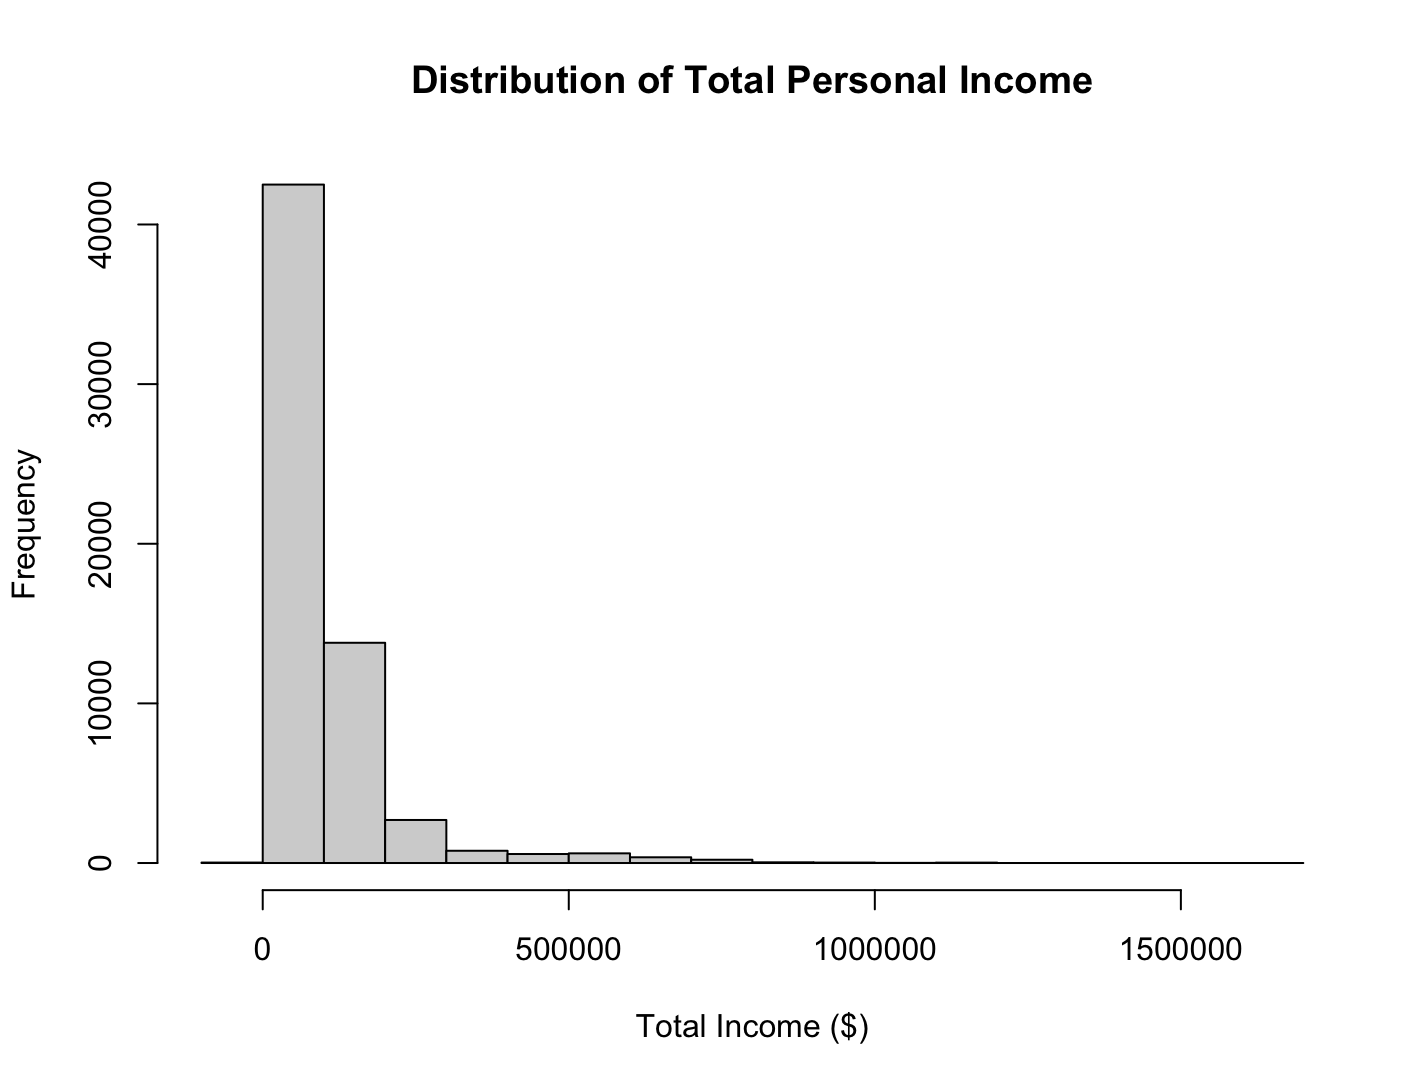
\includegraphics[width=\textwidth]{../figures/pre/Income_raw.png}
    \captionof*{figure}{\textit{Untransformed Income Distribution}}
\end{minipage}
\begin{minipage}{0.49\textwidth}
    \centering
    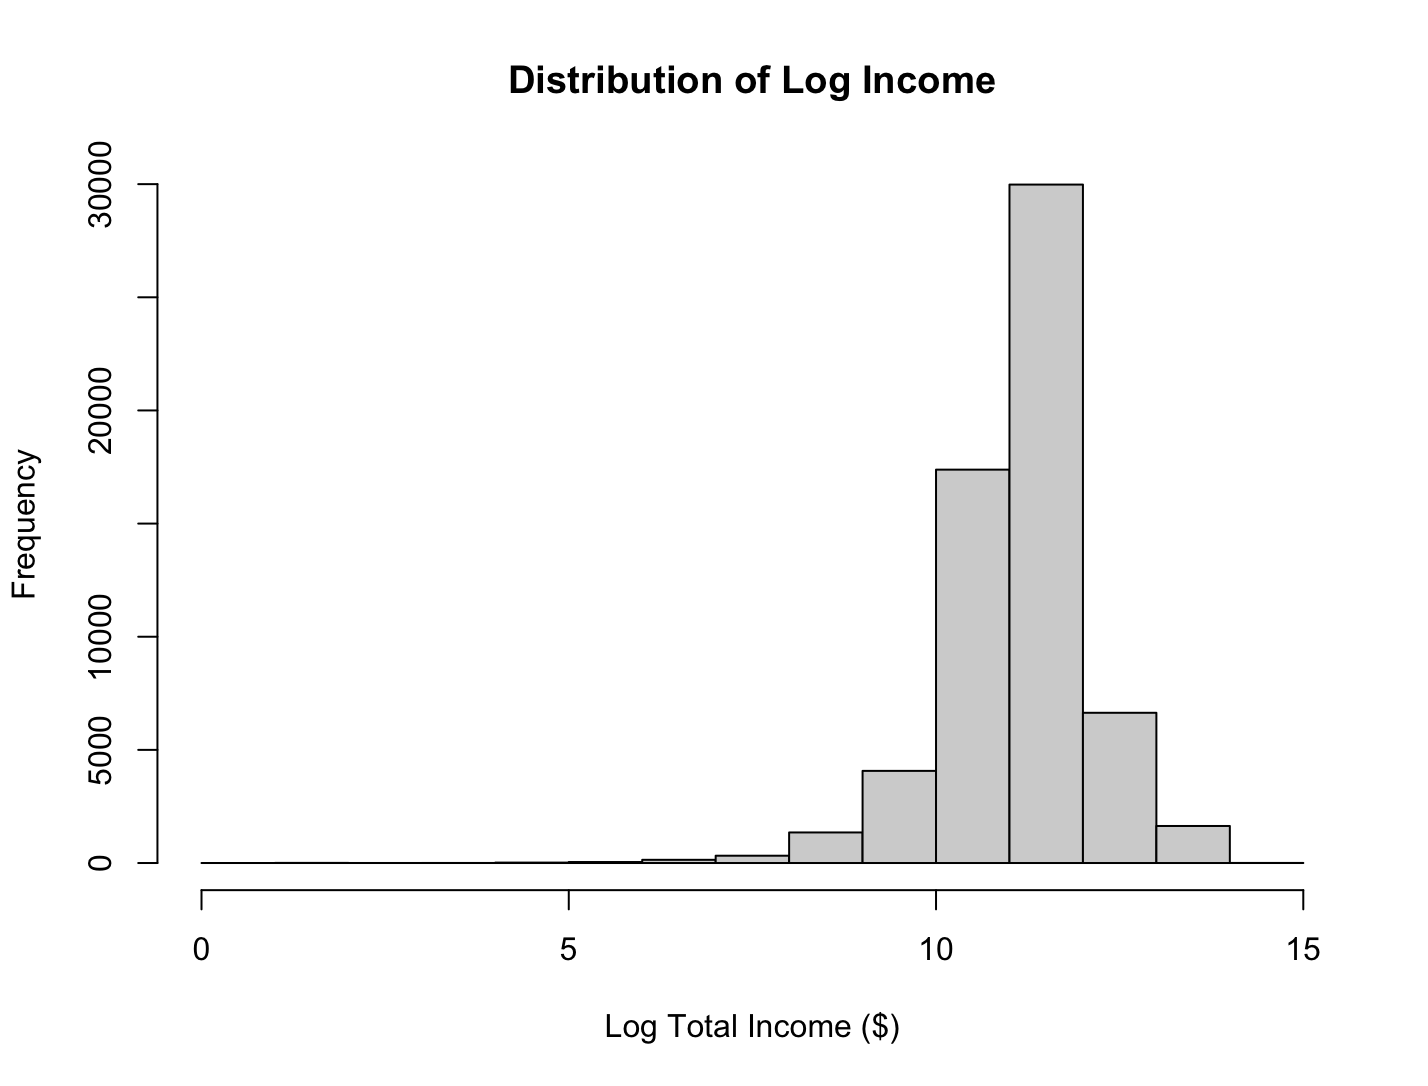
\includegraphics[width=\textwidth]{../figures/pre/Log_income.png}
    \captionof*{figure}{\textit{Log-transformed Income Distribution, the outcome}}
\end{minipage}
\vfill
\begin{minipage}{0.49\textwidth}
    \centering
    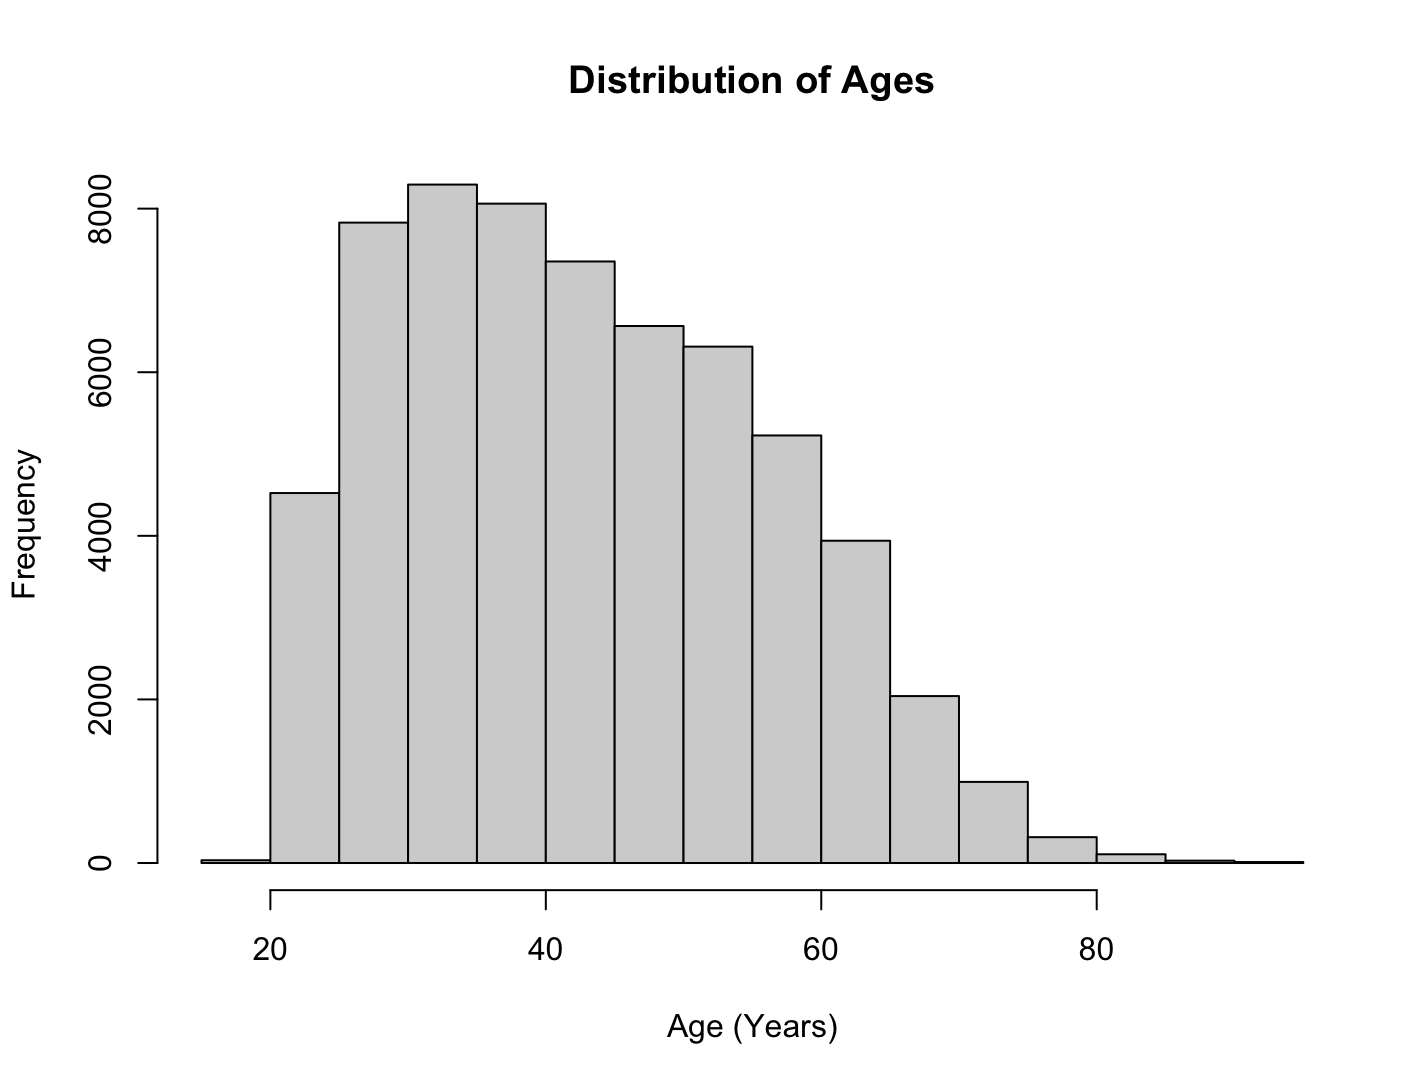
\includegraphics[width=\textwidth]{../figures/pre/age_plot.png}
    \captionof*{figure}{\textit{Age Distribution}}
\end{minipage}
\begin{minipage}{0.49\textwidth}
    \centering
    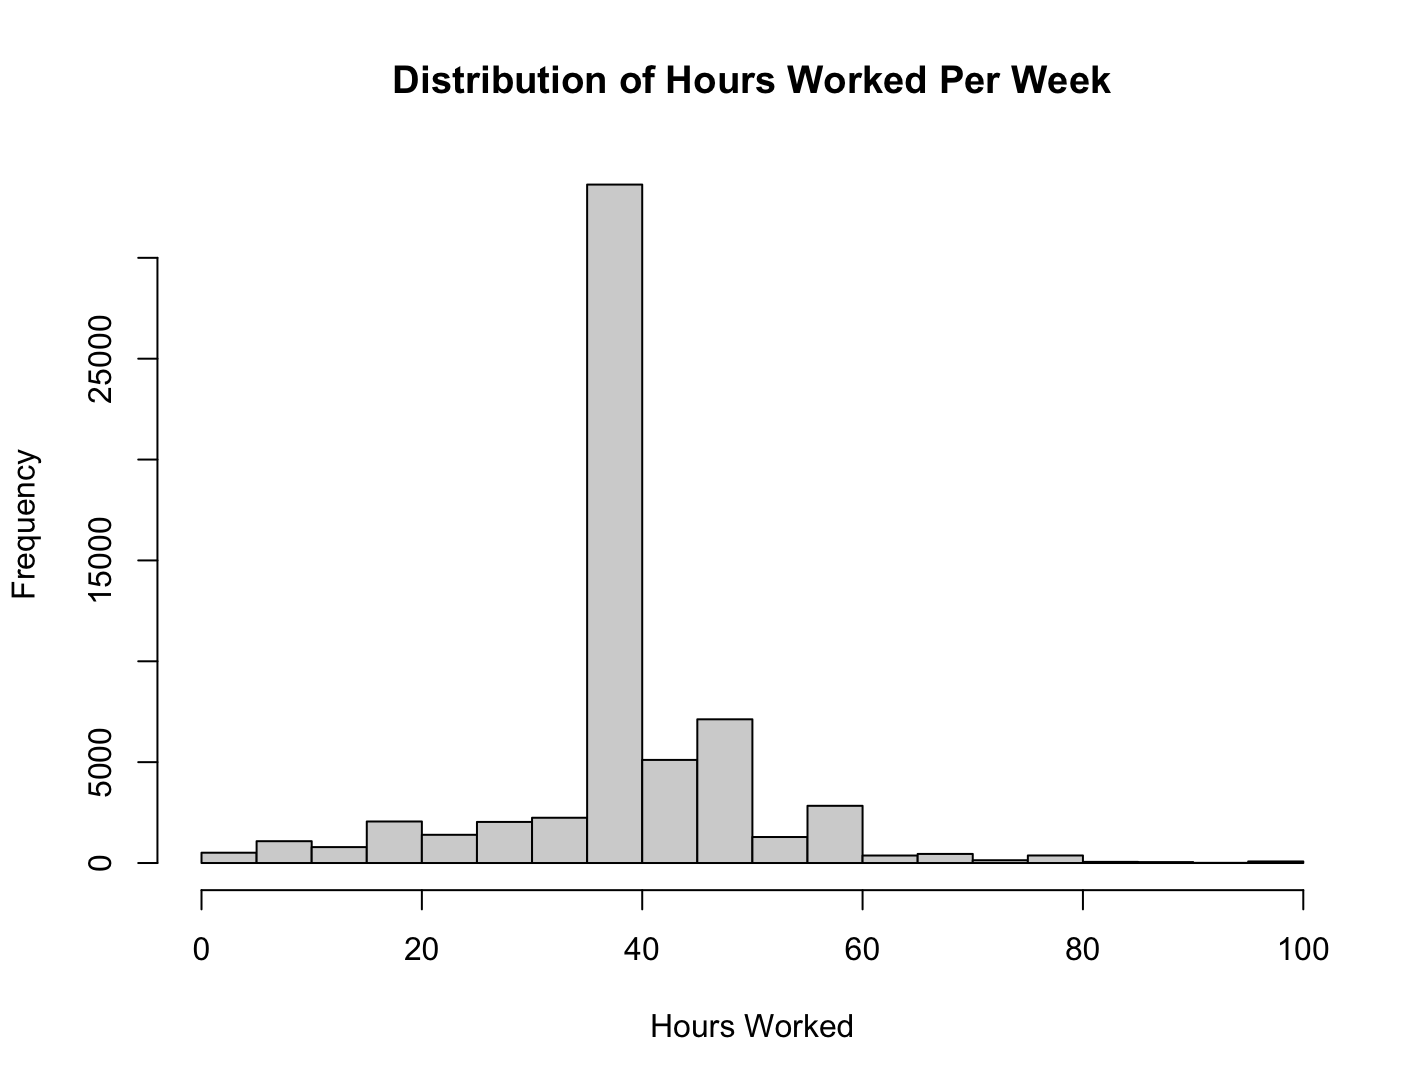
\includegraphics[width=\textwidth]{../figures/pre/hours_worked_plot.png}
    \captionof*{figure}{\textit{Hours Worked Distribution}}
\end{minipage}






    
\newpage
\subsubsection*{Categorical Variables}
    
    \begin{table}[ht]
    \centering
    \caption{Summary Statistics for Categorical Variables}
    \begin{tabular}{@{}lll@{}}
    \toprule
    Variable & Category & Proportion \\ 
    \midrule
    \multirow{2}{*}{SEX} & Female & 50.88\% \\
                         & Male & 49.12\% \\
    \midrule
    \multirow{9}{*}{RACE} & American Indian or Alaska Native & 0.42\% \\
                          & Black/African American & 8.62\% \\
                          & Chinese & 2.65\% \\
                          & Japanese & 0.37\% \\
                          & Other Asian or Pacific Islander & 7.56\% \\
                          & Other race, nec & 3.23\% \\
                          & Three or more major races & 0.70\% \\
                          & Two major races & 8.06\% \\
                          & White & 68.39\% \\
    \midrule
    \multirow{5}{*}{WORKREGION} & International & 0.05\% \\
                                & Midwest Region & 20.17\% \\
                                & Northeast Region & 22.73\% \\
                                & Other U.S. Territories and Special Areas & 0.77\% \\
                                & South Region & 32.36\% \\
                                & West Region & 23.92\% \\
    \midrule
    \multirow{13}{*}{DEGFIELD} & Arts and Design & 5.05\% \\
                               & Business and Industry & 22.55\% \\
                               & Communication and Media & 4.71\% \\
                               & Education and Teaching & 8.44\% \\
                               & Family and Consumer Studies & 0.72\% \\
                               & Health Sciences & 8.13\% \\
                               & Interdisciplinary Studies & 0.87\% \\
                               & Legal and Criminal Studies & 2.33\% \\
                               & Linguistics and Foreign Languages & 0.81\% \\
                               & Science and Environmental Studies & 2.14\% \\
                               & Social Sciences and Humanities & 21.42\% \\
                               & STEM & 22.82\% \\
                               & Technical and Vocational & 0.01\% \\
    \bottomrule
    \end{tabular}
\end{table}


\vfill
\begin{minipage}{0.49\textwidth}
    \centering
    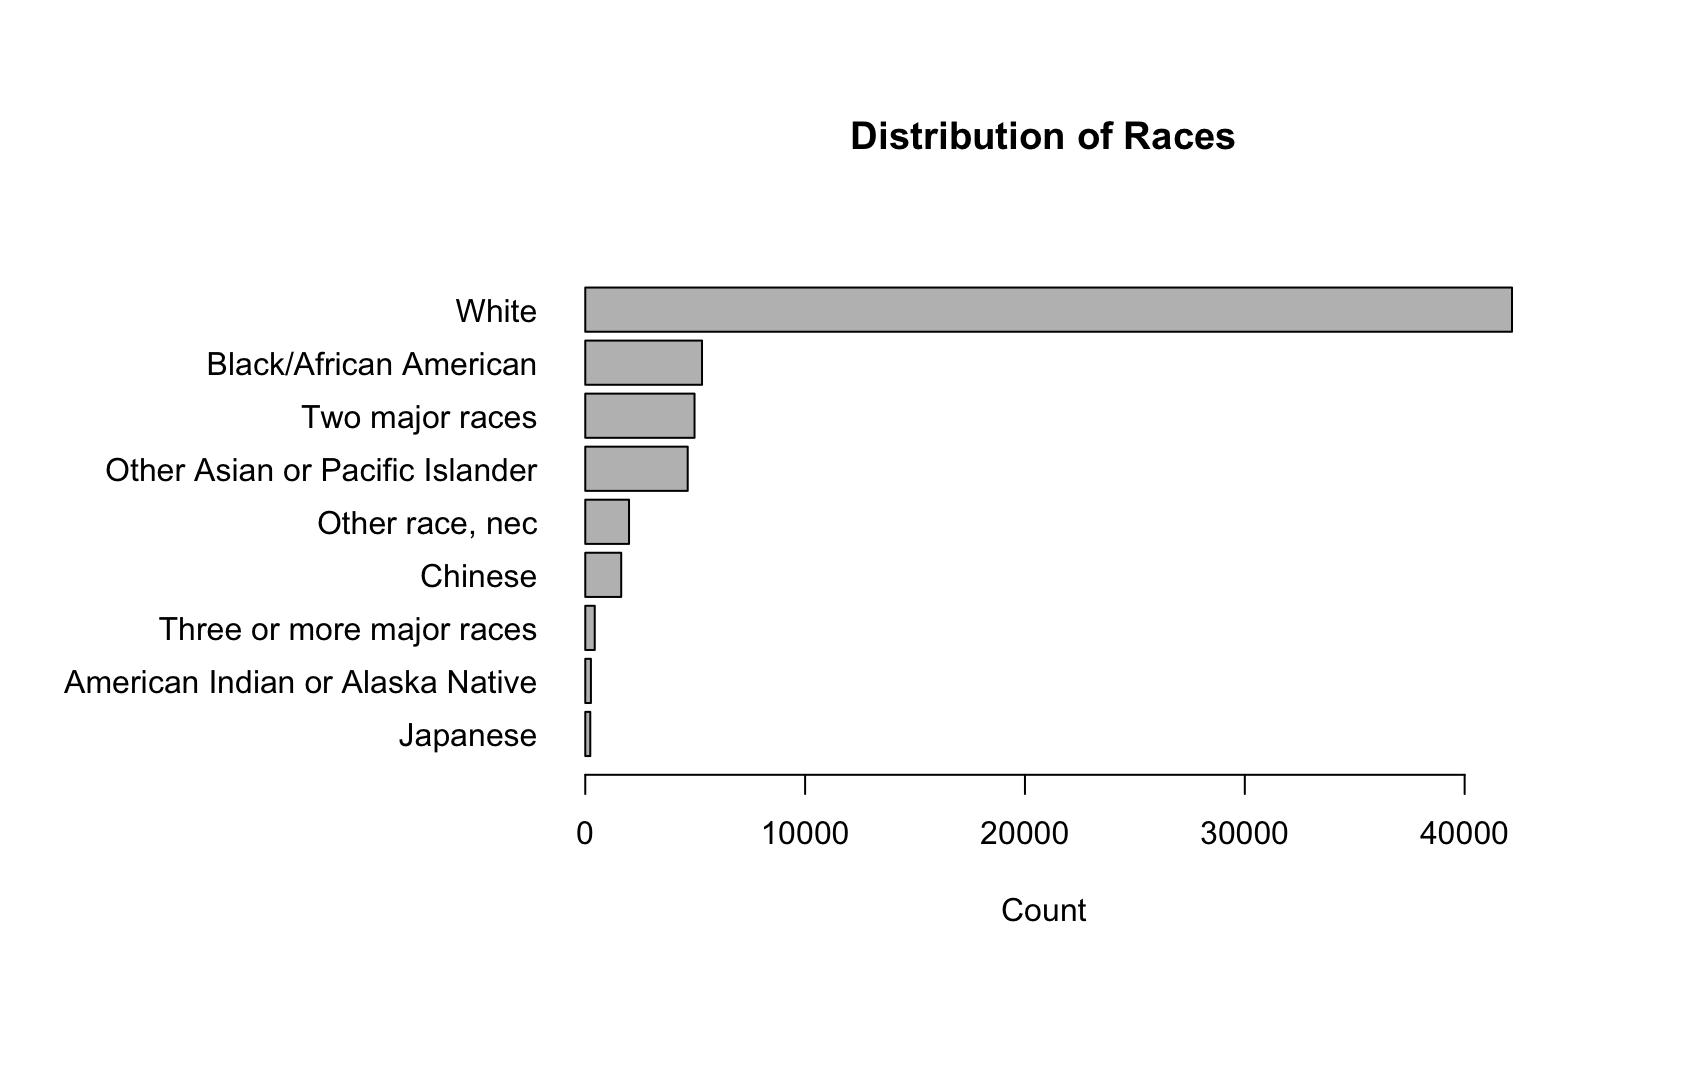
\includegraphics[width=\textwidth]{../figures/pre/race_plot.png}
    \captionof*{figure}{\textit{Race Distribution}}
\end{minipage}
\begin{minipage}{0.49\textwidth}
    \centering
    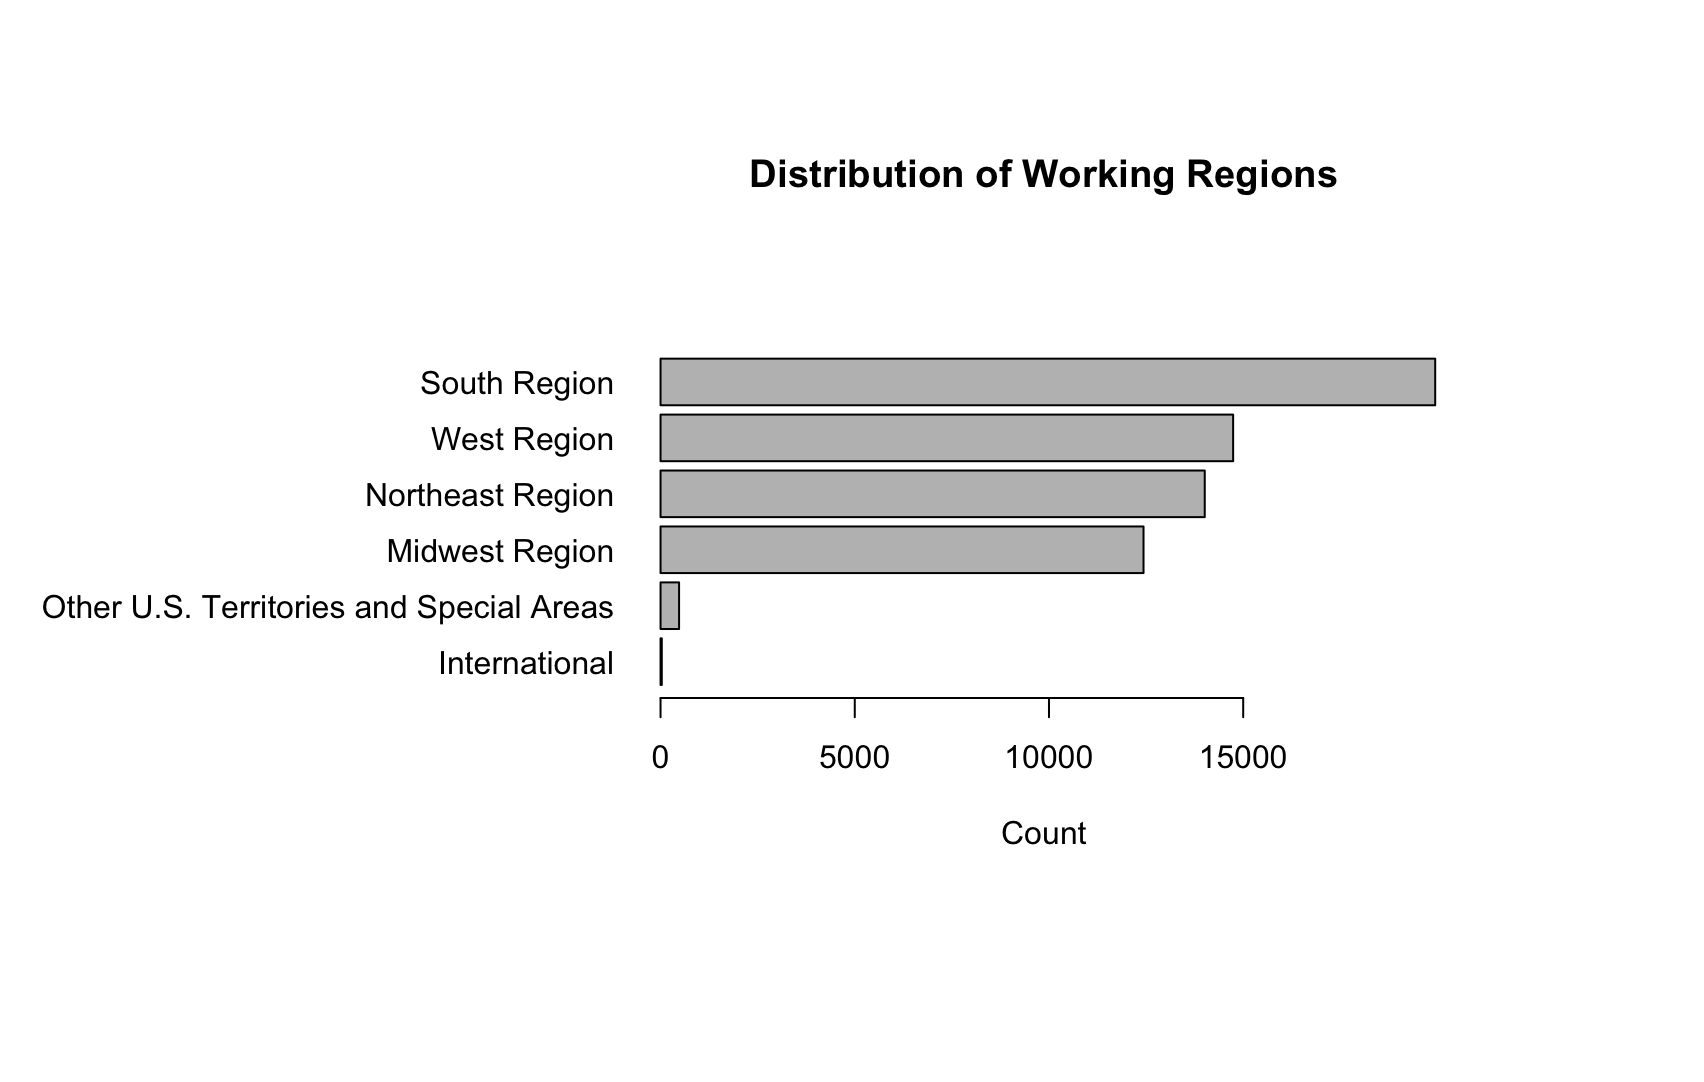
\includegraphics[width=\textwidth]{../figures/pre/work_region_plot.png}
    \captionof*{figure}{\textit{Work Region Distribution}}
\end{minipage}
\vfill
\begin{center}
    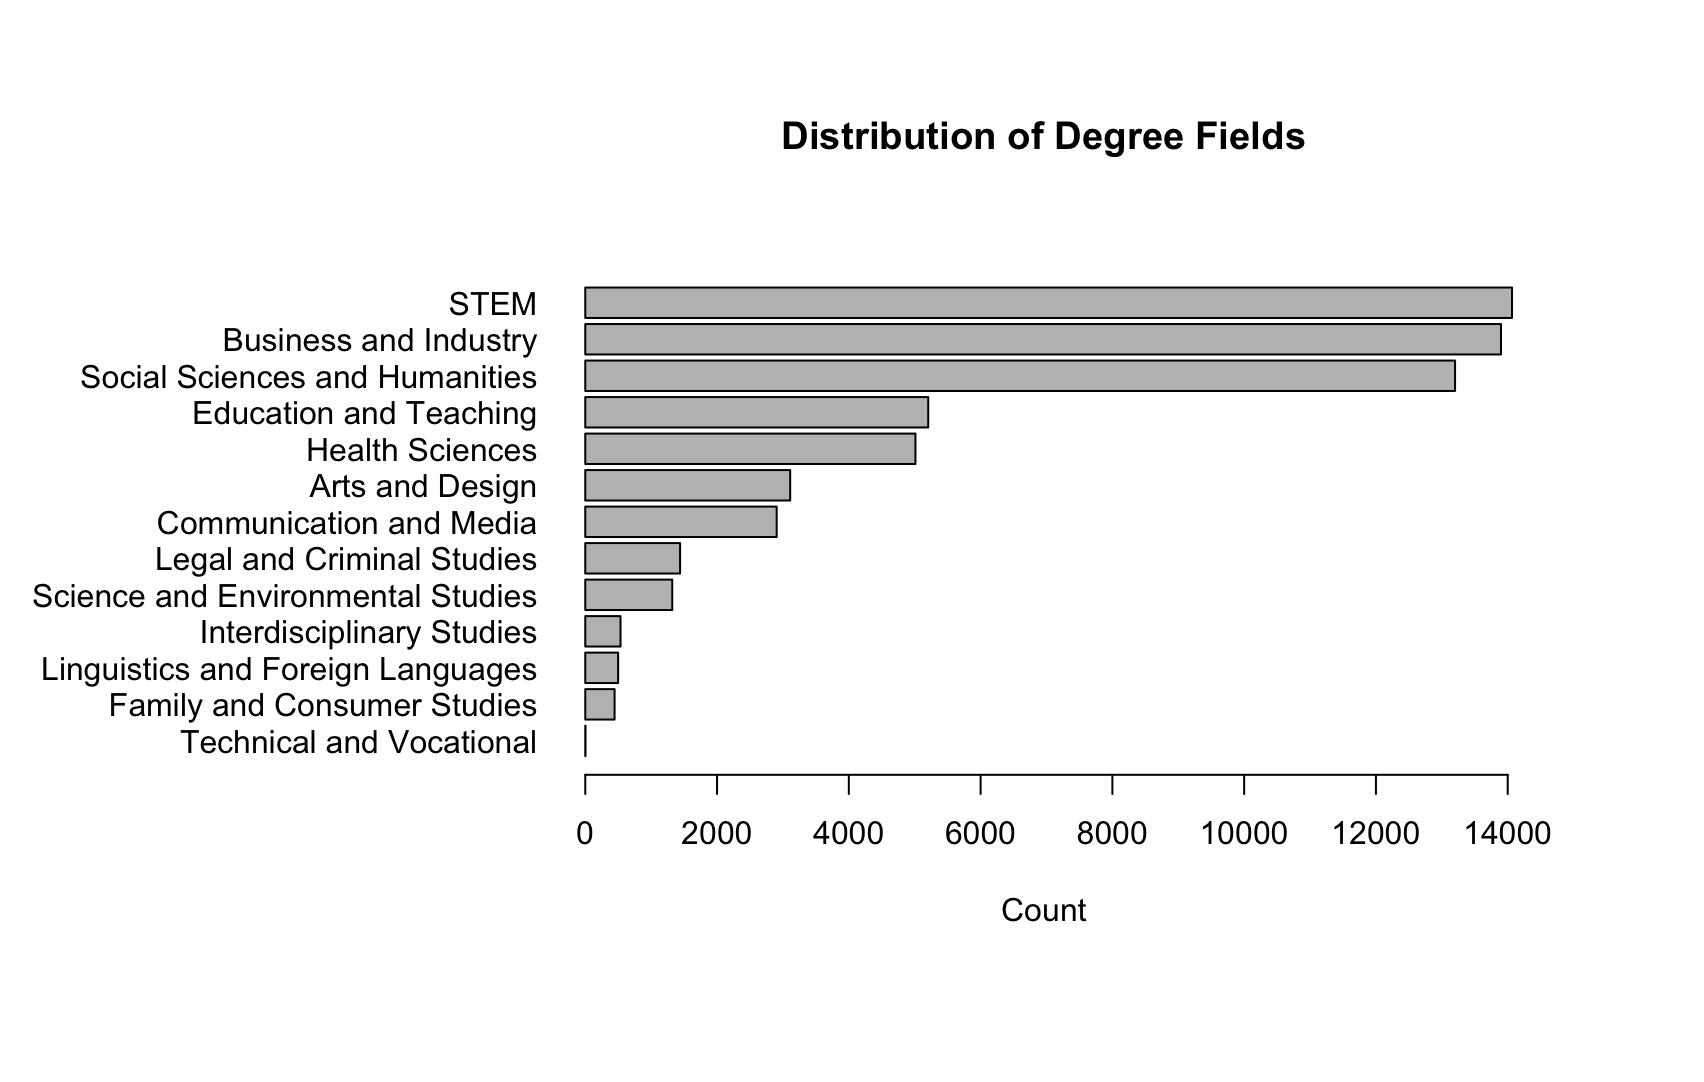
\includegraphics[width=0.8\textwidth]{../figures/pre/deg_field_plot.png}
    \captionof*{figure}{\textit{Degree Field Distribution}}
\end{center}
% \begin{minipage}{0.49\textwidth}
\newpage
\vfill
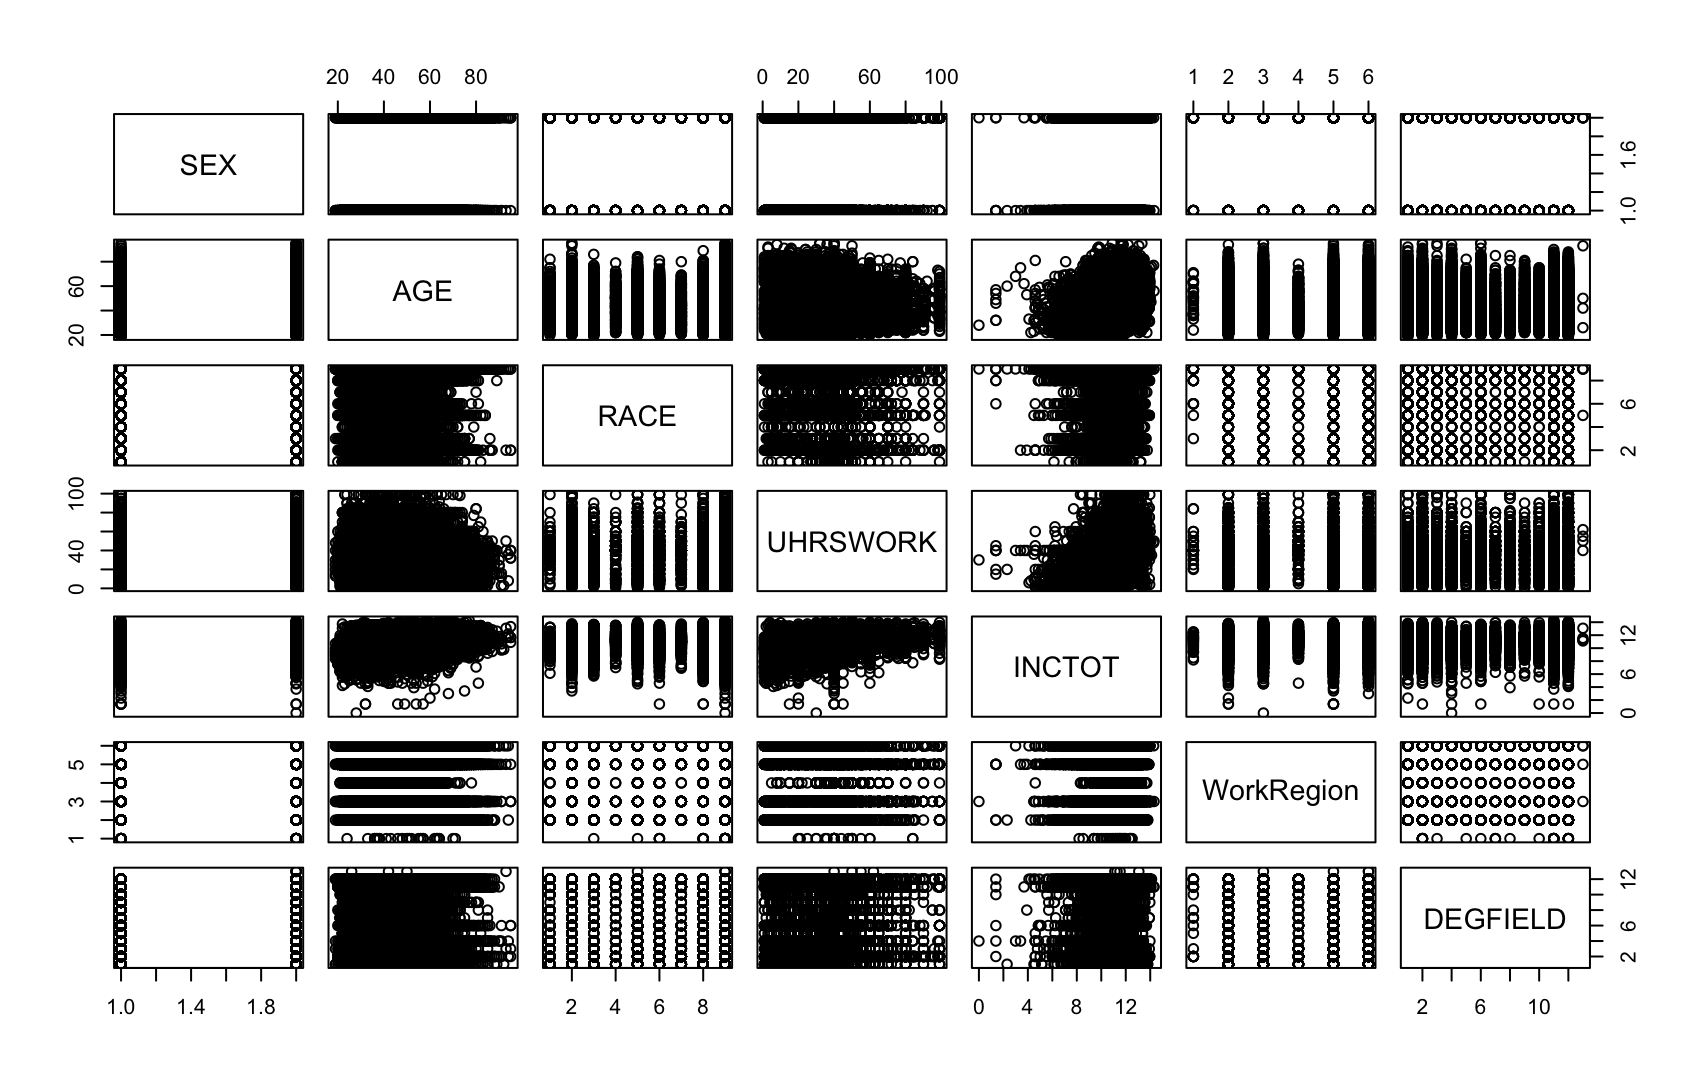
\includegraphics[width=\textwidth]{../figures/pre/scatter_matrix.png}
\captionof*{figure}{\textit{Feature Scatterplot matrix}}
\vfill

\end{custommargins}


\section*{Multivariate Regression Model}
We created the following multivariate regression model to study how individual income by sex, controlling for age, race, working region, hours worked per week, and degree field. 
\begin{equation*}
\begin{aligned}
\log(\text{INCTOT}) &= \beta_0 + \beta_1 \text{AGE} + \beta_2 \text{AGE}^2 + \beta_3 \text{SEX Male} \\
&+ \beta_4 \text{RACE American Indian or Alaska Native} + \beta_5 \text{RACE Black/African American} \\
&+ \beta_6 \text{RACE Chinese} + \beta_7 \text{RACE Japanese} + \beta_8 \text{RACE Other Asian or Pacific Islander} \\
&+ \beta_9 \text{RACE Other race, nec} + \beta_{10} \text{RACE Three or more major races} \\
&+ \beta_{11} \text{RACE Two major races} + \beta_{12} \text{DEGFIELDArts and Design} \\
&+ \beta_{13} \text{DEGFIELDBusiness and Industry} + \beta_{14} \text{DEGFIELDCommunication and Media} \\
&+ \beta_{15} \text{DEGFIELDEducation and Teaching} + \beta_{16} \text{DEGFIELDFamily and Consumer Studies} \\
&+ \beta_{17} \text{DEGFIELDHealth Sciences} + \beta_{18} \text{DEGFIELDInterdisciplinary Studies} \\
&+ \beta_{19} \text{DEGFIELDLegal and Criminal Studies} + \beta_{20} \text{DEGFIELDLinguistics and Foreign Languages} \\
&+ \beta_{21} \text{DEGFIELDScience and Environmental Studies} + \beta_{22} \text{DEGFIELDSocial Sciences and Humanities} \\
&+ \beta_{23} \text{DEGFIELDTechnical and Vocational} + \beta_{24} \text{UHRSWORK} \\
&+ \beta_{25} \text{WorkRegion International} + \beta_{26} \text{WorkRegionMidwest Region} \\
&+ \beta_{27} \text{WorkRegionNortheast Region} + \beta_{28} \text{WorkRegionOther U.S. Territories and Special Areas} \\
&+ \beta_{29} \text{WorkRegionWest Region}
\end{aligned}
\end{equation*}
% \noindent

We decided to include \texttt{Age\textsuperscript{2}} to capture the dynamic that income is expected to increase at a decreasing rate, maximizing mid career, then declining with retirement. The reference value for the categorical variable was chosen as the sub-group with the largest number of responses. For example, STEM was chosen as the reference group for the \texttt{DEGFIELD} variable since it is the most frequent degree field. The coefficients and p-vales of this regression model were used to determine whether there exists a significant difference in personal income among men and women. The predictive accuracy of this model was evaluated using Cross Validation and R-squared metrics

\section*{Results}


\begin{table}[ht]
    \centering
    \begin{tabular}{rrrrr}
      \hline
     & Estimate & Std. Error & t value & Pr($>$$|$t$|$) \\ 
      \hline
    (Intercept) & 8.1278 & 0.0365 & 222.80 & 0.0000 \\ 
      AGE & 0.0647 & 0.0016 & 40.07 & 0.0000 \\ 
      I(AGE\verb|^|2) & -0.0005 & 0.0000 & -29.54 & 0.0000 \\ 
      SEX: Male & 0.2390 & 0.0071 & 33.80 & 0.0000 \\ 
      RACE: American Indian or Alaska Native & -0.3328 & 0.0512 & -6.49 & 0.0000 \\ 
      RACE: Black/African American & -0.2013 & 0.0121 & -16.66 & 0.0000 \\ 
      RACE: Chinese & 0.0490 & 0.0209 & 2.35 & 0.0189 \\ 
      RACE: Japanese & -0.1265 & 0.0545 & -2.32 & 0.0203 \\ 
      RACE: Other Asian or Pacific Islander & -0.0327 & 0.0129 & -2.53 & 0.0116 \\ 
      RACE: Other race, nec & -0.3016 & 0.0189 & -15.97 & 0.0000 \\ 
      RACE: Three or more major races & -0.1037 & 0.0397 & -2.61 & 0.0091 \\ 
      RACE: Two major races & -0.1449 & 0.0124 & -11.72 & 0.0000 \\ 
      DEGFIELD: Arts and Design & -0.3587 & 0.0164 & -21.86 & 0.0000 \\ 
      DEGFIELD: Business and Industry & -0.1501 & 0.0099 & -15.11 & 0.0000 \\ 
      DEGFIELD: Communication and Media & -0.2423 & 0.0169 & -14.35 & 0.0000 \\ 
      DEGFIELD: Education and Teaching & -0.3978 & 0.0138 & -28.73 & 0.0000 \\ 
      DEGFIELD: Family and Consumer Studies & -0.3599 & 0.0397 & -9.06 & 0.0000 \\ 
      DEGFIELD: Health Sciences & -0.0466 & 0.0140 & -3.34 & 0.0009 \\ 
      DEGFIELD: Interdisciplinary Studies & -0.1375 & 0.0362 & -3.80 & 0.0001 \\ 
      DEGFIELD: Legal and Criminal Studies & -0.2685 & 0.0228 & -11.78 & 0.0000 \\ 
      DEGFIELD: Linguistics and Foreign Languages & -0.2031 & 0.0374 & -5.43 & 0.0000 \\ 
      DEGFIELD: Science and Environmental Studies & -0.3006 & 0.0237 & -12.69 & 0.0000 \\ 
      DEGFIELD: Social Sciences and Humanities & -0.2142 & 0.0102 & -20.99 & 0.0000 \\ 
      DEGFIELD: Technical and Vocational & -0.0024 & 0.4094 & -0.01 & 0.9952 \\ 
      UHRSWORK & 0.0313 & 0.0003 & 103.31 & 0.0000 \\ 
      WorkRegion: International & -0.3112 & 0.1449 & -2.15 & 0.0317 \\ 
      WorkRegion: Midwest Region & -0.0078 & 0.0094 & -0.82 & 0.4107 \\ 
      WorkRegion: Northeast Region & 0.1321 & 0.0091 & 14.53 & 0.0000 \\ 
      WorkRegion: Other U.S. Territories and Special Areas & 0.3509 & 0.0380 & 9.23 & 0.0000 \\ 
      WorkRegion: West Region & 0.1481 & 0.0091 & 16.25 & 0.0000 \\ 
       \hline
    \end{tabular}
\end{table}
Recall that setting all of the above race coefficients to zero, indicates the predicted log income of a white individual.
The same is true for the degree field coefficients, where setting all of them to zero indicates the predicted log income of a STEM degree holder.
Similarly, setting the work region coefficients to zero indicates the predicted log income of an individual working in the south region.


\begin{custommargins}{2cm}{2cm}
\subsection*{Residual Spread}
% \vfill
\begin{minipage}{0.49\textwidth}
    \centering
    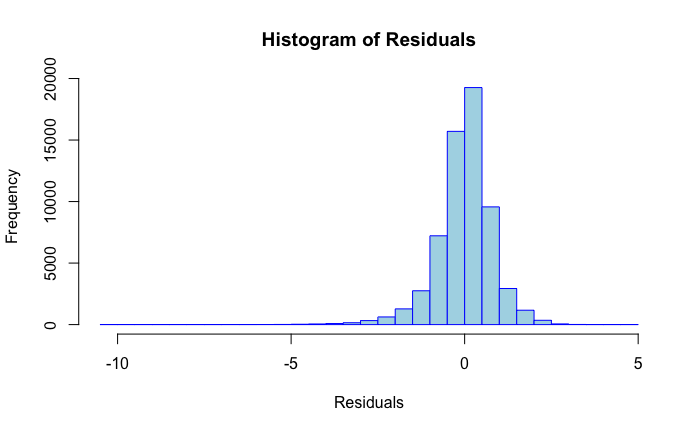
\includegraphics[width=\textwidth]{../figures/post/hist-k-foldcv.png}
    \captionof*{figure}{\textit{Residual Histogram}}
\end{minipage}
\begin{minipage}{0.49\textwidth}
    \centering
    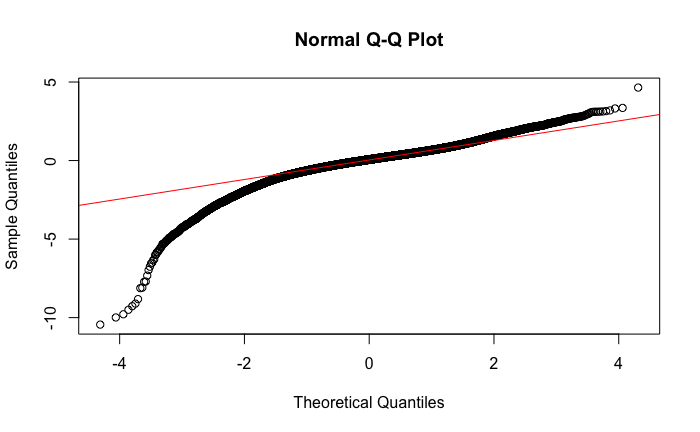
\includegraphics[width=\textwidth]{../figures/post/qq-k-foldcv.png}
    \captionof*{figure}{\textit{Residual Quantile-Quantile Plot}}
\end{minipage}
\vfill
\begin{minipage}{0.49\textwidth}
    \centering
    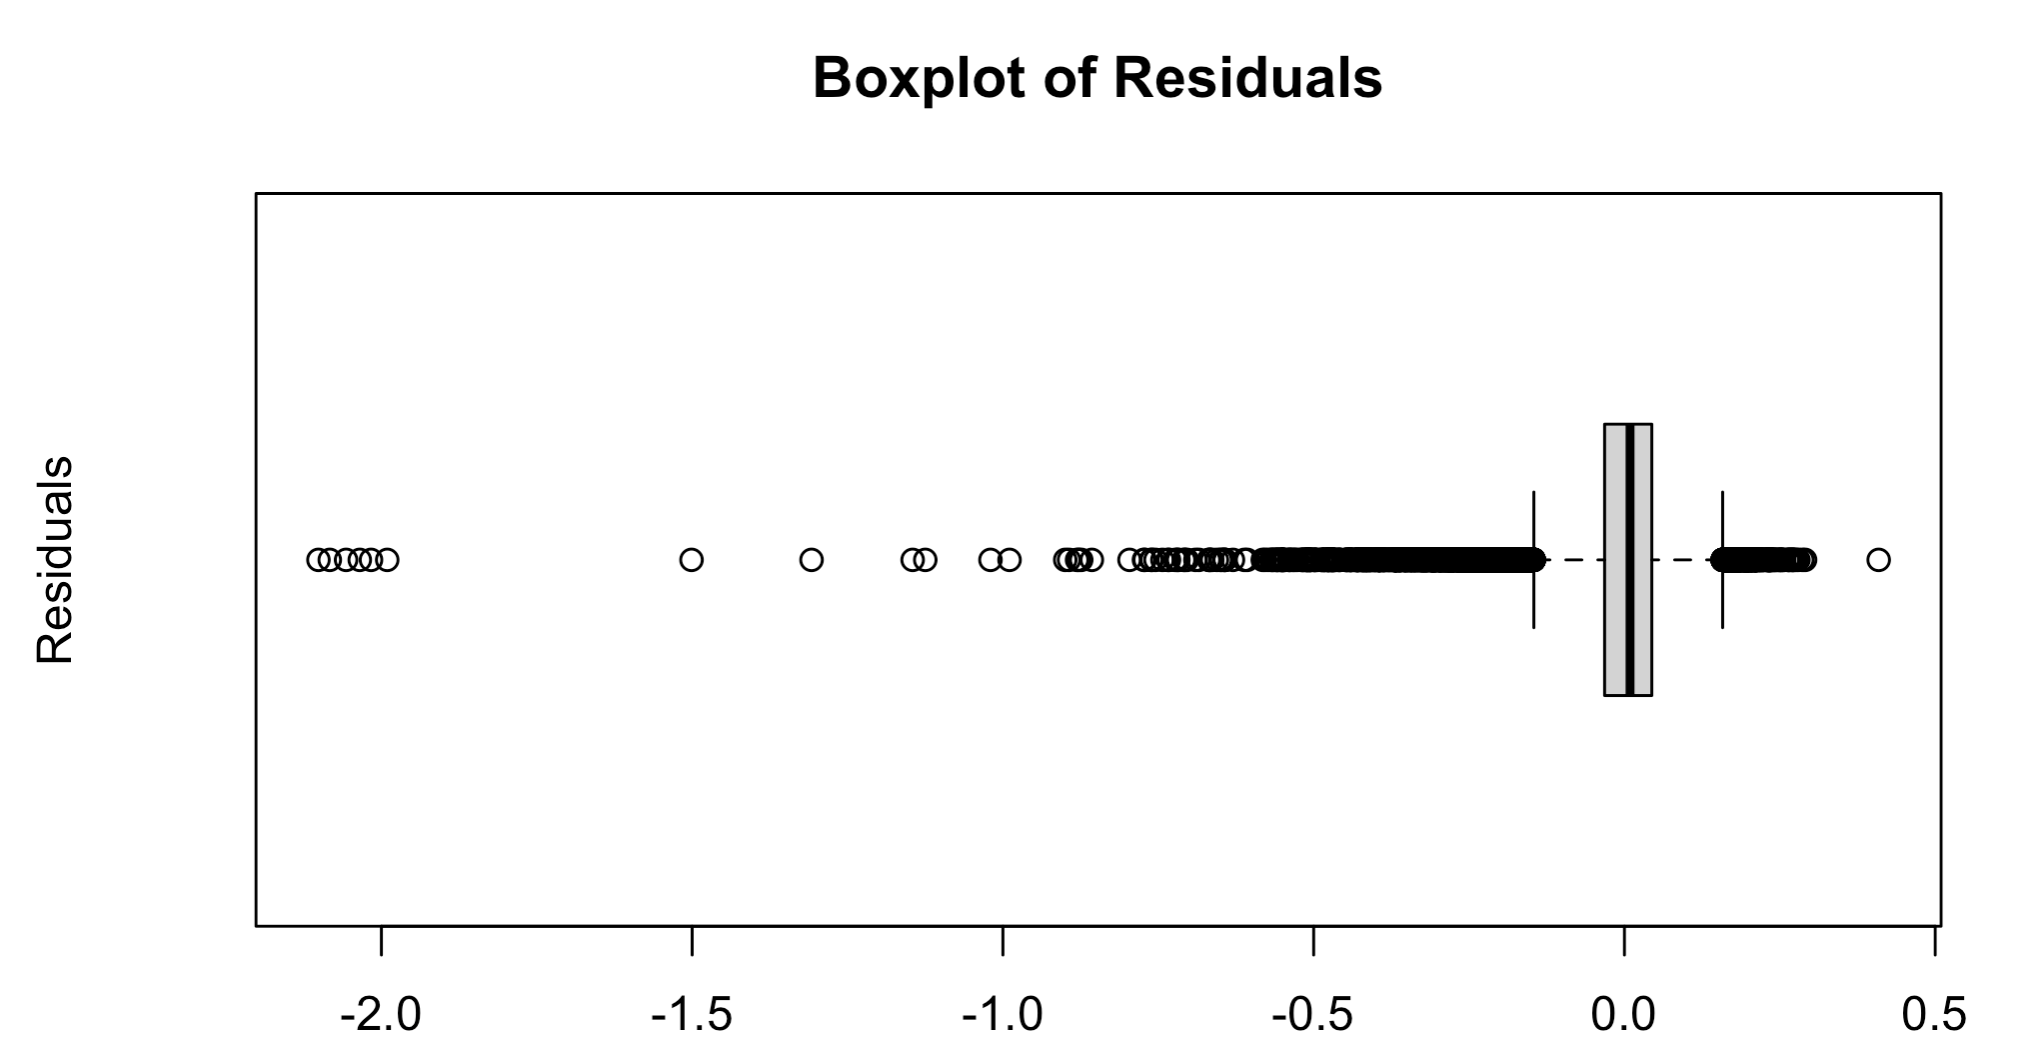
\includegraphics[width=\textwidth]{../figures/post/residual-box.png}
    \captionof*{figure}{\textit{Residual Boxplot}}
\end{minipage}
\begin{minipage}{0.49\textwidth}
    \centering
    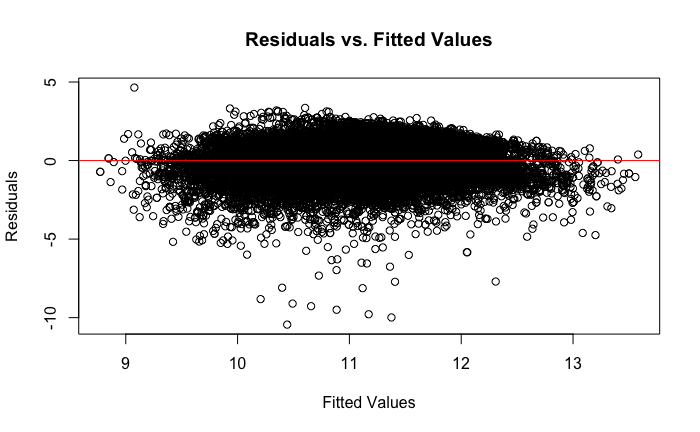
\includegraphics[width=\textwidth]{../figures/post/residualvsfitted-k-foldcv.png}
    \captionof*{figure}{\textit{Normalized Residuals vs Fitted Values}}
\end{minipage}
\vfill
\end{custommargins}
Our findings suggest that the residuals of our model are not normally distributed, therefore limiting the inferential power of our conclusions.
The quantile-quantile residual plot suggests a distribution with deviation from the reference line, which represents a normal distribution.

The plot of normalized residuals vs fitted values suggests that the residuals do not have constant variance.
This suggests that our estimates of the true $\beta$ coefficients are biased. However, due to the large sample size, and the standard errors of the $\hat{\beta}$ coefficients
, we can still conclude that the positive or negative relationship between the variables and income is both accurate and statistically significant.

The boxplot and histograms of residuals further suggests their non-normality. The presense of outliers in the lower values of \texttt{log(INCTOT)} suggests that our model may be underestimating the income of individuals with lower income.
This leads into the issues that the presense of high-income individuals has on our model and raises questions about the reliability of our seemingly good sample data.

%perhaps some more model metrics
\subsubsection*{Model Metrics}
\begin{table}[h]
    \centering
    \begin{tabular}{lr}
    \toprule
    \textbf{Statistic} & \textbf{Value} \\
    \midrule
    Residual Standard Error & 0.8194 \\
    for Degrees of Freedom= & 49256 \\
    \midrule
    Multiple R-squared & 0.2826 \\
    Adjusted R-squared & 0.2822 \\
    F-statistic & 669.1 \\
    DF for F-statistic & 29 and 49256 \\
    p-value & $< 2.2 \times 10^{-16}$ \\
    Root Mean Square Error & 0.8143115 \\
    \bottomrule
    \end{tabular}
    \caption*{Summary Statistics of the Regression Model}
\end{table}

The residual standard error was calculated to be 0.8194, which is the average difference between the observed and predicted values.

\subsubsection*{Cross-Validation}
For our results, we performed k=10 stratified cross-validation to compute the root mean square error.

The root mean square error (RMSE) is 0.8143, which is the square root of the average of the squared differences between the observed and predicted values. In dollar amounts, the exponentiated transformation
of the residual standard error and RMSE are \$2.27 and \$2.26, respectively. This suggests that our model's predictions are only off by around \$2.26 on average,
a relatively small amount. Our model is significant, given the chosen cutoff of $\alpha=0.05$ and the model's p-value.

\section*{Discussion}
Interestingly, our results reveal significant differences in income associated with race, degree field, working region, and gender.
Keeping everything else constant, the coefficient for \texttt{SEXMale} is 0.2390, which suggests the presence of a nontrivial gap in income between men and women.
This coefficient corresponds to a 26.9\% male advantage in pay or as more commonly stated, a .79 cents to the dollar wage gap.
Given the large sample size, the significance of the coefficient, and the large value of the coefficient, we conclude that the wage gap is statistically present
and due to discrimination as we control for several other key determinants of income.

In this report, we set the significance level of $\alpha = 0.05$, adhering to commonly accepted standards in statistical hypothesis testing. With this
level of $\alpha$, we find that the only three variables with no statistical effect on income to be \texttt{DEGFIELD: Technical and Vocational} and \texttt{WorkRegion: Midwest Region} at least when compared to the reference groups of \texttt{STEM} and \texttt{South Region}, respectively.

We find that individuals are paid differently per region. The coefficients of our model suggest that working in U.S. territories and special areas or the West Region are generally paid more on average compared to the other regions.
We find that working in International Region is associated with the lowest income, holding every other variable constant. These findings are interesting yet difficult to interpret and rely on as the International Region only represents 0.05\% of our sample data, which is itself 0.01\% of the whole survey.
Yet overall, changing working region does have a significant and meaningful impact on income, perhaps not as much as other variables, but this proves to be a good control for what we're trying to measure. This is especially true
as we use potentially global data for our analysis.

The field of degree impacts the income of individuals more than any other variable used in our model. This is not surprising, as we value various types of work differently.
Expectedly, we see that the highest paid degree fields are Business and Industry, Health Sciences, and STEM, with STEM, our reference variable, being the highest paid on average.
The lowest paid degree fields are Arts and Design, Education and Teaching, and Family and Consumer Studies. These findings are particulrly interesting in our discussion, as these are traditionally
female-dominated roles, while STEM and Business are traditionally male-dominated.

The strong correlation between working in Education and Teaching and being a female suggests that this variable may have absorbed some of the estimated disparity in pay, a potential explanation for the negative coefficient.
The National Center for Education Statistics reports that in 2022, 77\% of public school teachers are female and notes that "women were paid significantly less than their male counterparts"\cite{public-school}.
This suggests the presense of a pay gap in a different way: through choice of career field. However, this is a desired outcome of our model since we want to quantify the difference in pay while controlling for these choices.
The difference in pay between men and women due to carreer choice is an interesting and important topic, but it is not the focus of our study.

Additionally, we find that every measured race has a significant impact on an individual's income, suggesting racial disparities in pay. The largest disparity is between American Indian or Alaska Native and White individuals, with the former earning only 71.7\% as much as a white individual. 
It was important to include race in the discussion of income as a significant disparity in pay occurs across different races. This is a well-documented phenomenon, and our model confirms this.

The measure of typical hours worked per week was a crucial control variable in our model.
The coefficient of 0.0313 suggests that for every additional hour worked per week, an individual's yearly income increases by 3.18\%. This relationship is probably non-linear for low values such as 1 hour typically worked, but our input data suggests that 75\% of observations work at least 40 hours per week, which is standard for full-time employment.
Due to the impactfulness of this coefficient, it's relatively large corresponding coefficient, and the large range of values it takes on, this may be the most important determinant of income in our model.

Finally, we report an Adjusted R-squared value of 0.2822, indicating that our model explains approximately 28.22\% of the variance in income.
This suggests that while our model is informative, we fail to explain even half of the residual variance in income.
In their article, published by the Social Science Research Network, Peterson K. Ozili "examines the acceptable R-square in social science empirical modelling with particular focus on why a low R-square model is acceptable in empirical social science research." \cite{ozili}.
They explain that the goal of social science research is to understand rather than predict, and argues that a low R-squared value is acceptable on the condition that "that some or most of the predictors or explanatory variables are statistically significant"\cite{ozili}.

% do our negative residuals have something in common?
\subsection*{Discussion of Model Assumptions}
Our model seems to violate two out of the four general assumptions of linear regression. We meet the condition of linearity by transforming our input features
and the outcome variable and our residual show independence.

The residuals of our model are not normally distributed, which violates the normality of residuals assumption. This is evident by the histogram and qq-plot of residuals.
This potentially limits how significant our factors are in explaining income, as the p-values rely on this assumption. However, their very small values suggests that our model is still significant.
Perhaps if the p-values were closer to $\alpha$, we would have to reconsider the model.

Additionaly, we violate the assumption of homoscedasticity, as the residuals do not have constant variance. This is evident by the residual vs fitted plot.
This implies that our estimates of the true $\beta$ are biased, and that our model may have underestimated the standard errors of each coefficient.


\subsection*{Limitations}
While our model explains a significant portion of the variance in income (Adjusted R-squared = .2822), there is still a substantial amound of unexplained variance.

There are several other factors that our model does not measure in the discussion of income. Firstly, are economic factors such as inflation, interest rates, and the overall economic health of the economy. 
Depending on complex macro-economic relationships, these factors significantly impact individuals differently. Furthermore, a group of people may deal with a worse economy in 
a better way; for example, males may have a higher income in a poorer economy due to having better job security, furthering income disparities.
Alternatively, the government may provide additional stimulus to certain disatvantaged groups during a recessionary period, which could also alter income disparities.
That is to say, that economic factors affect people differently which potentially explains some of the unexplained variance in our model or altering our estimate of the wage gap.

Other potential factors that could influence the discussion of a wage gap include
having children, having a disability, or being married. And while controlling for typical hours worked per week does capture some of the impact of having children or being married, it cannot fully capture the
full impact on worker productivity our life outlook.
Women may work the same amount of hours before and after having children, but may not take advantage of opportunities to advance their career. We cannot fully describe how our model would change if we considered these variables,
but we acknowledge that these additional factors are significant enough as to alter the results of our findings.

Additionally, our model could've benefitted from additional interactions such as an interaction between race and gender. This would allow us to measure potentially compounding disparities in pay that occur
when an individual may be of two disadvantaged groups. The explanatory power of our model and a more complete understanding of the wage gap could be improved by including this interaction.

Furthermore, the impact of the COVID-19 pandemic is unmeasured in our model. As we use data from after the pandemic, patterns that we've encountered in our data may be different
from the patterns that existed before the pandemic and studies of that time. And while our findings are similar from the pre-pandemic era, national working patterns are not.
We find that working hours and region are still significant predictors of income, but these have changed since after the pandemic. More people work remotely than they every have, and they can do so from across the country.
Working hours, therefore, are measured with less reliability due to more instances of self-reporting as opposed to a standardized work clock. Also, where we live may not define our pay as much as it has.

This is to say that controlling for these variables may not be as adequate as they are not as influential as they once were. This implies that other variables may be absorbing the impact of these variables, potentially altering our estimate for the differences 
in gender pay. We must refine how we measure income and the factors that influence it to better understand the gap.

\subsection*{Further Considerations}
Further research could be done to understand other factors that may influence income, as mentioned in the limitations section. The better
we may explain income, the better we can attribute the wage gap to discrimination. This could also be done by including more interactions in our model, such as an interaction between
race and gender, or between degree field and working region. This would allow us to measure the compounding effects of being in several disatvantaged groups for further insight.

Additionally, further research could be done to understand the wage-gap across different wealth classes. Anecdotal evidence suggests that the wage gap is more pronounced in lower income brackets, but
this is not that well understood. This would provide crucial insight into where the gap is most prevalant and how we could address it.

Finally, social forces change across time, and the wage gap may be different in the future. Fixing social issues requires continuous research and analysis in order to monitor the effects of 
policy changes and societal shifts. This analysis should be done in the future and by several different groups to ensure that results are consistent, reliable, and relevant.


\clearpage
\begin{thebibliography}{9}
    \bibitem{HRfH}
    Chen, Z., Zhang, Y., Luo, H. et al. Narrowing but persisting gender pay gap among employees of the US Department of Health and Human Services during 2010–2018. \textit{Human Resources for Health}, \textbf{19}(65), 2021.
    \bibitem{BLSarticle}
    Toossi, Mitra. A Century of Change: The U.S. Labor Force, 1950-2050, May 2002, \href{www.bls.gov/opub/mlr/2002/05/art2full.pdf}{link}.
    \bibitem{issuebrief}
    Understanding the Gender Wage Gap, Women’s Bureau, Department of Labor, Mar. 2023, \href{www.dol.gov/sites/dolgov/files/WB/equalpay/WB_issuebrief-undstg-wage-gap-v1.pdf}{link}. 
    \bibitem{DallasFed}
    Liu, Sitian, and Yichen Su. “The Geography of Jobs and the Gender Wage Gap.” Federal Reserve Bank of Dallas, Working Papers, vol. 2020, no. 2028, Oct. 2020, \href{https://doi.org/10.24149/wp2028}{doi}. 
    \bibitem{public-school}
    “NCES Blog | August 26. 2022.” Nces.ed.gov, \href{nces.ed.gov/blogs/nces/2022/08/26/default}{link}.
    \bibitem{ozili}
    Ozili, Peterson K. “The Acceptable R-Square in Empirical Modelling for Social Science Research.” Papers.ssrn.com, 5 June 2022, \href{papers.ssrn.com/sol3/papers.cfm?abstract_id=4128165}{link}.
    \bibitem{census}
    Guzman, Gloria, and Melissa Kollar. “Income in the United States: 2022.” United States Census Bureau, United States Census Bureau, 12 Sept. 2023, \href{www.census.gov/library/publications/2023/demo/p60-279.html}{link}.
    
\end{thebibliography}

\section*{Code}
\subsection*{Replication}
You can run our code and replicate our results by running the R markdown file \texttt{final-code.Rmd} in version 4.3.2

\end{document}